\documentclass{sig-alternate-10pt}

\usepackage{amsmath}
\usepackage{amssymb}
\usepackage{xcolor}
\usepackage{times}
\usepackage{xspace}
\usepackage{listings}
\usepackage{algorithm}
\usepackage[noend]{algpseudocode}
\usepackage{tikz}
\usetikzlibrary{arrows,automata,positioning}

\newcommand{\todo}[1]{\textcolor{red}{[TODO: #1]}}
\newcommand{\ratul}[1]{\textcolor{blue}{[ratul: #1]}}
\newcommand{\ryan}[1]{\textcolor{green}{[ryan: #1]}}

\newcommand{\sysname}{{\small \sf Propane}\xspace}

\newcommand{\para}[1]{\paragraph*{\textbf{#1}}}

\newcommand{\set}[1]{\ensuremath{\{ #1 \} }}
\newcommand{\abs}[1]{\ensuremath{ \lvert #1 \rvert }}
\newcommand{\path}[2]{ #1 \mapsto \ensuremath{#2} }

\begin{document}

\special{papersize=8.5in,11in}
\setlength{\pdfpageheight}{\paperheight}
\setlength{\pdfpagewidth}{\paperwidth}

\title{Toward Centrally Programming Distributed Control Planes}
\author{Paper \#XXX}

\maketitle

%\category{CR-number}{subcategory}{third-level}
%% general terms are not compulsory anymore,
%% you may leave them out
%\terms
%term1, term2
%\keywords
%keyword1, keyword2
\textbf{Abstract---}
Networks are notoriously difficult to configure correctly. 
Operators typically rely on local configuration of individual devices running 
distributed control plane protocols to achieve network-wide objectives. 
Managing implicit dependencies between device configurations and properly accounting for failures makes 
a network operator's work particularly difficult. 
%
The recent move towards software-defined networking has been motivated, in part, 
by the simplicity of the centralized model, where a controller directly manages 
individual devices rather than letting them manage themselves. However distributed 
protocols have many important advantages in scalability,
latency and fault tolerance over the completely centralized approach.
%
In this paper, we describe a new system -- \sysname, which allows an operator to specify a high-level, 
centralized routing policy declaratively, but then to compile it to a purely distributed 
implementation, which uses the BGP routing protocol to run on existing, commodity hardware. 
%
Propane allows operators to describe the types of paths traffic may (or may not) take 
through the network, as well as relative preferences (or backups) between paths. 
%
Network policies compiled with \sysname are guaranteed to implement the correct routing policy regardless of the number of failures, if possible.  If this is not possible, the compiler notifies the user at compile time rather than as the network is in 
operation.
%
\sysname also takes the centralized model one step further by unifying inter and intra-domain routing. Operators can specify routing policy for an autonomous system by programming against the abstraction that they can control any route in the wider internet.
%
We have implemented a compiler for \sysname and evaluated it against several real-world configurations for data centers and core backbone networks. We demonstrate the \sysname compiler can scale to 
topologies with thousands of routers.

\section{Introduction}
\label{sec:introduction}

It is well-known that network configuration is highly error
prone and that such errors can lead to costly network
downtime~\cite{mahajan+:bgp-misconfiguration,feamster+:rcc,batfish}.
For instance, a recent misconfiguration led to an hour-long, nation-wide outage for Time Warner's backbone network~\cite{time-warner}; and a major BGP-related incident makes international news every few months~\cite{bgpmon}.

%For instance, in the context of BGP, Mahajan~~\cite{mahajan+:bgp-misconfiguration}
%estimated that 200-1200 prefixes suffered from
%misconfiguration each day and that close to 3 in 4 of all
%new prefix advertisements were the result of misconfiguration.
%Moreover, these misconfigurations sometimes cause significant network downtime for
%individual networks~\cite{time-warner} or even broader internet connectivity problems~\cite{routing-instability,mahajan+:bgp-misconfiguration}.
%\dpw{Note that \cite{time-warner} and I am not sure about the specifics of the problem there
%or what exactly was misconfigured.  It is also unclear if our language really helps with the
%``broader internet connectivity problems'' however, I thought that adding some specific examples
%would help make the intro more compelling.  Feel free to rewrite.}

One reason for network configuration being onerous is that device configuration languages are low-level and several configuration elements must be kept consistent (e.g., interface addresses) for the device to behave as intended.

Another, more fundamental reason is the semantic mismatch between the intended high-level
policies and the low-level device-by-device configurations.  In particular,
many policies involve network-wide properties---prefer a certain neighbor,
never announce a particular destination externally,
use a particular path only if another fails---but configurations describe the behavior of
individual devices.
%
Operators must manually decompose network-wide policy into device-level behaviors, such that their interactions satisfy the high-level objectives.
%
Ensuring policy-compliance through this manual decomposition is challenging under normal
circumstances and even more so in the face of failures. Some decompositions that work correctly
in failure-free environments, violate key constraints when failures occur.
%
As a result, many network configuration problems are only revealed after failures~\cite{batfish},
sometimes making a bad situation worse.

To reduce configuration errors, many practitioners have a adopted a template-based
approach~\cite{hatch,thwack}, in which common configuration patterns are captured as parameterized templates.
 While templates help ensure certain kinds of consistency across devices, they do not
bridge the
semantic divide between network policies and device-level configuration.
They do not provide fundamentally different abstractions
from existing configuration languages.

Software-defined networking (SDN) and its abstractions 
are, in part, the research
community's response to the difficulty of maintaining policy
compliance through distributed interaction of individual
devices~\cite{sdn-languages}. Indeed, instead of organizing networks
around a distributed collection of devices that compute forwarding tables through
mutual interactions, the devices are told how to
forward packets by a centralized controller. The controller is responsible for ensuring that the
paths taken are compliant with operator specifications.
%Researchers
%have developed increasingly sophisticated languages that let operators
%specify desirable network paths~\cite{x,y,z} which are then translated
%to forwarding tables at runtime.

The centralized control planes of SDN, however, are not a panacea.
%
They require careful design and engineering to be robust to failures at scale---one must ensure that all devices can communicate with the controller at all times, even under arbitrary combinations of failure~\cite{x,y,z}. To address this challenge, many researchers are beginning to explore
multi-controller networks, with interacting controllers, thus bringing back distributed
control planes~\cite{x,y,z} and their current programming difficulties.  However, academic
language design and implementation efforts have not kept pace.  For instance, work on
experimental SDN languages
such as Frenetic~\cite{frenetic}, Flowlog~\cite{flowlog}, Vericon~\cite{vericon}, Merlin~\cite{merlin}, NetKAT~\cite{netkat}, and Kinetic~\cite{kinetic}, to
name a few, has not yet shown how to implement fault tolerant
multi-controller systems that support their abstractions efficiently.

In this paper, we ask if it is possible to program distributed control planes using network-wide policies.
Operators should be able to directly express network-wide policies, which are automatically decomposed into individual device configurations. The resulting forwarding behavior, which emerges through device interactions, must be policy-compliant under all possible failures.
If successful, this approach would combine easy programmability of centralized control planes and failure robustness of distributed control planes.
%
More pragmatically, it would help many networks that, for the foreseeable future, will continue to use a distributed control plane, due to the difficulty of migrating to SDN or the inherent scalability and failure-robustness of distributed control.

Through \sysname, our system that includes a language and a compiler, we demonstrate the feasibility of programming distributed control planes. We focus on BGP, a common and highly flexible way to implement distributed control planes, and show how to automatically generate router BGP configurations from network-wide policies.

We face two challenges in designing \sysname that differ from designing a system for programming data planes~\cite{x,y,z}. The first is policy specification itself---specifying network {\em policies} is different from specifying network {\em paths}.
%
The specification must compactly capture behavior under all possible failures. Since there is no controller at runtime, the routers must be programmed ahead of time, based on the specification, to handle failures.
%
Further, many policies naturally under-specify paths (e.g., "prefer paying neighbors" is not a concrete path).
%
\sysname addresses this specification challenge by allowing operators to express {\em path preferences}, where preference describes a set of valid paths and less-preferred options are taken only when a higher-preference options are unavailable.

The direct nature of \sysname specifications brings up the second challenge, of compiling them to router configurations.  We must compute the sets of paths represented by the intersection of multiple preferences and topology, compute which ones can be honored under a given failure scenario, and ensure policy compliance under all possible failure cases. We handle this challenge by compactly capturing policy and topology in a {\em product graph} and developing efficient algorithms that operate on this graph.

We evaluate \sysname by using it to encode policies of real backbone and data center networks.

\todo{new intro is not complete}



\section{Background on BGP}
\label{sec:background}

We focus on BGP as it is the most common and flexible way to implement distributed control planes today. Before delving into the details of our work, we provide here relevant background on BGP.

BGP is a path vector protocol that connects autonomous systems (ASes). An AS has one or more routers controlled by the same administrative entity. ASes exchange routing announcements with their neighbors. Each announcement has a destination IP prefix and some attributes (see below), and it indicates that the sending AS is willing to carry traffic to that prefix from the receiving AS. (Traffic flows in the opposite direction, from announcement receivers to senders.)

When an AS receives an announcement from a neighbor, it is processed by import filters that may drop the announcement or modify some attributes. If multiple announcements for the same prefix survive import filters, the router selects the best one based on local policy, expressed in terms of route attributes. This route is then used to send traffic to the destination. It is also advertised to the neighbors, after passing them through neighbor-specific export filters that may stop the announcement or modify some attributes.

A few route attributes are notable. The AS-path attribute accompanies all announcements and it has the ordered list of ASes that the announcement has traversed thus far. While AS-path attribute has a global meaning, some attributes are meaningful only within an AS or between neighboring ASes.  Two such attributes are communities and multi-exit discriminator (MED). Communities are opaque, string attributes that ASes use to color incoming routes on different criteria (e.g., ``entered on West Coast"). They can also be used to signal to neighbors about how the announcement should be handled (e.g., do not export it further). MEDs are used when an AS has more than one link to a neighboring AS. They are numeric values that signal to the receiving AS which link the sender prefers to receive traffic on. 

The route selection process assigns a {\em local preference} to each route that survives the import filters. Routes with higher local preference are preferred. For routes with equal preference, other factors such as AS path length, MEDs, internal routing cost, are considered in order. Because they are considered first in the selection process, they This preference can be based on any route attribute. It can also be based on the sending neighbor, which is a common practice.
 
 , or other existing attributes.  Local preference is an internal attribute that is not carried beteeen the first criterion in selecting the best route and higher numbers are assigned to preferred routes. BGP conside

aggregation




\section{Motivation}
\label{sec:motivation}

We motivate our work by describing the current practice in network configuration. In traditional networks with distributed control planes, the operators' goal is to generate the configuration of individual devices based on their desired policy. This configuration dictates the behavior of a device, how it exchanges routing information with neighbors and how it filters and ranks that information. The collective behavior of the devices should implement the desired policy.

Device configuration languages are low-level and indirect. For instance, instead of allowing operators to express directly the paths they want through the network, they require operators to specify metrics that result in those paths; instead of allowing operators to express directly the types of traffic to not carry through the network, they require operators to select and program an appropriate filtering mechanism (e.g., BGP import or export filters, null routing,  access control lists) and instantiate it on topologically appropriate devices; instead of allowing operators to directly specify that they prefer BGP neighbors in a certain order, they require operators to program local preferences and multi-exit discriminators (MED) at each router and ensure that the numbers are consistent across routers.

In many networks today, device configurations are generated manually by operators, without the support of many automated tools. It is easy to see the problems with this approach, such as typos, inconsistency across devices, and no guarantees of policy compliance.

To reduce such problems, some networks use a template-based approach. Configuration templates abstract certain constants into variables (e.g., instead of concrete community value, they may contain a variable {\small \sf{\$$BadNeighbor$)}} and may use a device vendor-neutral syntax. Operators manually generate the templates and use tools to translate them into device configuration, by replacing variables with appropriate constants using a database of network information.

 %and replacing vendor-neutral constructs with their vendor-specific counterparts.

%In practice, most networks use a hybrid of templates and manual generation of device configuration. Templates are used for standardized and common configuration elements across devices and the result is manually tweaked to obtain the exact desired network behavior.

While templates avoids some pitfalls of the fully manual approach, they too are far from ideal. The fundamental issue is the semantic mismatch between desired policies and the level of abstraction of templates. While many policies are network-wide (e.g., prefer customer networks, or never announce a route to a certain prefix to external neighbors), templates are device-level. Operators must still manually decompose network-wide policies into device-level policies that can produce the desired network-wide behavior.
This decomposition is not always straightforward and ensuring policy-compliance can be hard, especially in the face of failures. We illustrate this point using two examples based on policies that we have seen in practice.

\begin{figure}[t!]
\centering
\includegraphics[width=\columnwidth]{figures/example1}
\caption{Creating router-level policies is difficult.}
\label{fig:example1}
\end{figure}


\example{1}

Consider the backbone network in Figure~\ref{fig:example1}. It has three neighbors, a customer $Cust$ , a peer $Peer$, and a provider $Prov$. The policy of this network is shown on the right. Per commercial relationships, it prefers the neighbors in a certain order ($P1$) and does not want to act as a transit between Peer and Prov ($P2$). It prefers to exchange traffic with Cust over $R1$ rather than $R2$ because $R2$ is a more expensive link ($P3$). To guard against another AS "hijacking" prefixes owned by Cust, it only sends traffic to those prefixes if Cust is on the AS path ($P4$). Finally, to guard against Cust accidentally becoming a transit for Prov, it does not use Cust for traffic that will later traverse Prov ($P5$).

To correctly implement this network's policy, the operators must compute and assign local preferences such that preferences at Cust-facing interfaces $>$ Peer-facing interfaces $>$ Prov-facing interfaces. At the same time, the preference at $R2$'s Cust-facing interface should be lower than that at $R1$, but higher than that at Prov-facing interface. To fully realize $P2$, MEDs will have to be appropriately configured as well. To implement $P3$ and $P4$, the operators may assign communities that indicate where a certain routing announcement entered the network. Then, R4 must not announce to $Peer$ routes that have communities that correspond to the R2-prov link but must announce communities for the $R2$-Cust and $R1$-Cust links. Finally, to implement $P4$ and $P5$, the operators will have to compute and configure appropriate prefix- and AS-path-based filters at each router.

We can now see that devising correct configuration for real, larger networks will quickly become a nightmare. These networks will have many neighbors across multiple classes of commercial relationships, differing numbers of links per neighbor, along with several region-, neighbor- or prefix-based exceptions to the default policy. Templates only help to certain extent, e.g., by keeping preference and community values consistent across routers. The operators must still do much of the conceptually difficult work manually, in coming up with the templates themselves. \sysname enables a direct expression of the policies of such networks and compiles them automatically to individual router configurations.

\begin{figure}[t!]
\centering
\includegraphics[width=\columnwidth]{figures/example2}
\caption{Policy-compliance under failures is difficult.}
\label{fig:example2}
\end{figure}

\example{2}

If configuring policies for a fully functional network is difficult, doing so in a way that ensures policy compliance in the face of failures can be almost impossible. Consider the data center network in Figure~\ref{fig:example2} with routers organized as a fat tree and running BGP.\footnote{To scale and to simplify policy implementation, data center networks increasingly use BGP internally, with a private AS number per router~\cite{bgp-in-dc-rfc}.} The network has two clusters, one that hosts services that should be reachable globally and one that hosts that should be accessible only internally. This policy is enabled by using non-overlapping address space in the two clusters and ensuring that only the address space for the global services is announced externally. In addition, to reduce the number of prefixes that are announced externally, the global space is aggregated into one larger, less-specific prefix $P_G$. The semantics of aggregation in BGP is that the aggregate prefix is announced as long as the router has a path to even one sub-prefix.

The operator may decide that a simple way to implement the policy is to have X and Y: $i)$ not export externally what they hear from routers G and H since these routers border the cluster with local services; and $ii)$ announce what they hear from routers C and D and aggregate to $P_G$ if an announcement is subset of $P_G$. The appeal of this implementation is that X and Y do not need to be made aware of which prefixes are global versus local and IP address assignment can be done independently (e.g., new prefixes can be added to local services without updating router configurations).

However, this implementation is incorrect because it does not have the right behavior in the face of failures. Suppose links X--G and X--H fail. Then, X will hear announcements for $P_{l*}$ from C and D, having traversed from G and H to Y to C and D. Per policy implementation, X will start "leaking" these prefixes externally. Depending on the rationale for local services, this leak could impact security (e.g., if the services were sensitive) or availability (e.g., if the $P_{l*}$ prefixes are used for other services outside of the data center). This problem does not manifest without failures because then X has and prefers paths to $P_{l*}$ through G and H since they are shorter. A similar problem will happen if links Y--G and Y--H fail.
%\footnote{A different problem occurs when links X--C and X--D (or Y--C and Y--D) fail. X (Y) may stop announcing the global prefixes because they would be heard through G and H.}  
Link failures in data centers are frequent and it is not uncommon to have multiple failed links at a given time~\cite{dc-failure-study}.

\todo{remove if we do not discuss aggregation in the design}
To avoid this problem, the operator may decide to disallow paths with "valleys," i.e., those that go up, down, and back up again. This safeguard can be implemented by $X$ and $Y$ rejecting paths through the other. However, that creates a different problem in the face of failures---an aggregation-induced blackhole~\cite{xx}. Suppose links D--A and X--C fail. Now, X will hear announcements for $P_{g2}$ from D and will thus announce the $P_G$ externally. This announcement will bring to X traffic for $P_{g1}$ as well, but because of valley-free filtering, X does not have a valid route for $P_{g1}$ and will thus drop all traffic to it.

Thus, we see that devising configuration that ensures policy compliance in the face of failures is complex and error-prone. \sysname helps operators by implementing their high-level policy specification in a way that guarantees compliance under all failures if that is possible. Otherwise, it generates a compile-time error that informs them that the specification cannot be met. For aggregation, it will also provide a lower bound to operators on the number of failures under which aggregation will not result in blackholes.


%\subsection{OLD -- Overview}
%\todo{this subsection can be deleted once we have captured everything in it}
%
%Sources of bugs we fix. (It seems like the main advantage of our approach is not just fixing bugs though - it is easily describing high-level intention).
%Perhaps the best way to do this is by going through a bunch of examples in section 2 and showing how you could easily introduce bugs:
%
%\begin{itemize}
%	\item Out of sync, or copy paste errors due to replicated configs (never an issue due to centralized control)
%	\item Correct filtering to ensure no undesired traffic can flow through the network (e.g., best practices, like an AS should filter customers for their prefix, are implemented automatically )
%	\item Failures can easily lead to unexpected behavior (e.g., a datacenter failure scenario w/instability.)
%	\item Trying to do anything interesting, like get backups correct is difficult (e.g., setting up aggregation wrong)
%	\item Related to the last point, things like aggregation can introduce black holes. We have the information needed to prevent this
%\end{itemize}
%
%
%Possible Examples:
%\begin{itemize}
%	\item Basic datacenter with spine preference
%	\item Simple AS that prefers customers over peers over providers
%	\item Combined internal backup routing with preference based entrance into the network using aggregation.
%	\item Something like cold potato routing
%\end{itemize}


\section{Propane}
\label{sec:propane}


\sysname simplifies network configuration by automatically generating low-level BGP configurations from a high-level specification of the network's routing policy. 
%
The operator configures the network with the abstraction that he or she has centralized control over routing and uses a set of high-level constraints to describe the different routes traffic may (or may not) take and their relative preferences. 
%
The \sysname compiler generates BGP configurations for each device in the network that operate in a completely distributed fashion and are correct by construction -- automatically synthesizing import/export filters, local preference and MED attributes, and community tags to ensure policy compliance under all possible failure scenarios.
%
We now demonstrate \sysname by showing how to configure the networks from the previous examples.

\para{Example 1}

We now show how to write the routing policy for the backbone network in Section~\ref{sec:motivation}.


\para{Example 2}

Consider again the datacenter from Section~\ref{sec:motivation}. In this example, there are primarily three main concerns: (1) traffic for the prefix block allocated to each top-of-rack router can reach that router, (2) local services do not leak outside the datacenter, and (3) aggregation is performed on global prefixes to reduce churn in the network. 

\sysname allows us to decompose and specify each of these constraints in a modular fashion. The first constraint is about prefix ownership -- namely, that we only want traffic for certain prefixes to end up at a particular locations. The following definition in propane captures this intent:

\begin{lstlisting}[mathescape=true]
define Ownership = {
    $\path{p_{g1}}{end(A)}$
    $\path{p_{g2}}{end(B)}$
    $\path{p_{l1}}{end(E)}$
    $\path{p_{l2}}{end(F)}$
}
\end{lstlisting}

The constraints in the ownership task are read in a top-down fashion. Traffic for prefix $p_{g1}$ is only allowed to to follow paths that end at router A. Similarly, traffic not matching $p_{g1}$, but which matches $p_{g2}$ must end at router B and so on. 
%
To capture the second constraint, we can define another task for the core routing policy:

\begin{lstlisting}[mathescape=true]
define Routing = {
    $\path{p_{g*}}{any}$
    $\path{p_{l*}}{\neg enter(out)}$
    $\path{true}{exit(out)}$
}
\end{lstlisting}

The first line states that there is no restriction on how traffic must traverse the network for global prefixes. This means traffic for $p_{g*}$ may be sent either from other routers in the datacenter, or from external ASes. The second line ensures that traffic for local prefixes never enters the network from an outside location. This  guarantees that the services remain reachable only to locations internal to the data center.

Finally, we can combine these constraints logically to specify the network-wide policy:

\begin{lstlisting}[mathescape=true]
Ownership $\wedge$ Routing $\wedge$ agg($p_{agg}$, $in \rightarrow out$)
\end{lstlisting}


In addition to constraints on the shape of paths, \sysname allows the operator to specify constraints on the BGP control plane. Above, a constraint on aggregation is included to ensure that an aggregation for $p_{agg}$ is performed from locations inside the network to locations outside the network.

Once \sysname compiles the policy, it is guaranteed to hold under all possible failure scenarios. Similarly, it can check for aggregate-induced black holes up to $k$ failures. 





\section{Compilation}
\label{sec:compilation}





\subsection{Overview}

\begin{figure}[t!]
\centering
\includegraphics[width=\columnwidth]{figures/pipeline}
\caption{Compilation pipeline stages for Propane.}
\label{fig:pipeline}
\end{figure}

In this section we briefly describe our compilation strategy for \sysname. Figure~\ref{fig:pipeline} shows the 5 stage compilation pipeline to translate user-level \sysname policies into device-local BGP policies. The first stage of the pipeline involves simple rewriting rules and substitutions from the user-level languae into the core Regular Intermediate Representation (RIR). Policies in RIR are checked for well-formedness (e.g., never constraining traffic that does not enter the network), before being combined with topological information to obtain Product Graph Intermediate Representation (PGIR). The PGIR is a data representation that compactly captures the control flow of all BGP advertisements subject to the policy and topology restrictions. We develop efficient algorithms that operate over the PGIR to ensure policy compliance under failures, avoid BGP instability, and prevent aggregation-induced black holes. Once the compiler determines the PGIR for the policy is safe, the compiler uses a simple translation to an abstract BGP (ABGP) representation. To make configurations more readable for human operators, and to reduce the size of the resulting configurations, the \sysname compiler makes several passes over the ABGP form. Finally, vendor-specific adaptors can be added to \sysname to translate from ABGP to actual concrete configurations that go on the network devices.





\subsection{Regular IR (RIR)} 
\label{sec:rir}

The high-level language presented in Section~\ref{sec:propane} is just a thin layer on top of a core, regular-expression-based language for describing preference-based path constraints. Regular expressions are an expressive formalism that have been studied extensively for their utility in describing paths through graphs~\cite{bib:todo}, and applications to networks~\cite{bib:todo}. Our regular expression language differs from others by allowing operators to describe preferences between paths.

% grammar
\newcommand{\BNFALT}{\;\;|\;\;}
\newcommand{\hdr}[2]{\flushleft \chdr{#1}{#2}}
\newcommand{\chdr}[2]{\textbf{#1} {#2} \\ \centering}

\begin{figure*}
  \begin{minipage}[t]{.45\linewidth}
  \hdr{\large Syntax}{}
  \vspace*{-1\baselineskip}
  %
  \[ \begin{array}{rclr}
    \hline

     pol     &::=& p_1, \dots, p_n & \textit{constraints} \\
     p       &::=& t \mapsto r_1 \gg \dots \gg r_m & \textit{preferences} \\
     t       &::=& & \textit{test} \\
         &\BNFALT& true & \textit{true} \\
         &\BNFALT& \neg t & \textit{negation} \\
         &\BNFALT& t_1 \vee t_2 & \textit{disjunction} \\
         &\BNFALT& t_1 \wedge t_2 & \textit{conjunction} \\
         &\BNFALT& prefix = x & \textit{prefix test} \\
         &\BNFALT& comm = c & \textit{community test} \\
     r       &::=& & \textit{regular paths} \\ 
         &\BNFALT& n & \textit{AS number} \\
         &\BNFALT& in & \textit{internal loc} \\
         &\BNFALT& out & \textit{external loc} \\
         &\BNFALT& r_1 \cup r_2 & \textit{union} \\
         &\BNFALT& r_1 \cap r_2 & \textit{intersection} \\
         &\BNFALT& r_1 \cdot r_2 & \textit{concatenation} \\
         &\BNFALT& !(r) & \textit{path negation} \\
         &\BNFALT& r^* & \textit{repetition} \\
     l       &::=& r_1 \rightarrow r_2 & \textit{link pairs} \\
     cc     &::=& agg(x, l) \BNFALT tag(c, t, l) & \textit{control constraints} \\
  \end{array} \]

  \end{minipage}
  %
  ~~
  \vrule
  ~~
  %
  \begin{minipage}[t]{.5\linewidth}
  \hdr{\large Propane Expansions}{}
  \vspace*{-1\baselineskip}
  %
  \[ \begin{array}{rcl}
    \hline
    any           & = & out^* \cdot in^+ \cdot out^* \\
    internal      & = & in^+ \\
    external      & = & out^+ \\
    only(X)       & = & any \cap X^* \\
    never(X)      & = & any \cap (!X)^* \\
    through(X)    & = & out^* \cdot in^* \cdot X \cdot in^* \cdot out^* \\
    after(X)      & = & out^* \cdot (X \cap out) \cdot out^* \cdot in^+ \cdot out^* \\
    before(X)     & = & out^* \cdot in^+ \cdot out^* \cdot (X \cap out) \cdot out^* \\
    end(X)        & = & any \cap (\Sigma^* \cdot X) \\
    start(X)      & = & any \cap (X \cdot \Sigma^*) \\
    exit(X)       & = & (out^* \cdot in^* \cdot (X \cap in) \cdot out \cdot out^*) \cup \\
                  &        & (out^* \cdot in^+ \cdot (X \cap out) \cdot out^*) \\
    enter(X)      & = & (out^* \cdot out \cdot (X \cap in) \cdot in^* \cdot out^*) \cup \\
                  &        & (out^* \cdot (X \cap out) \cdot in^+ \cdot out^*) \\
    link(X,Y)     & = & any \cap (\Sigma^* \cdot X \cdot Y \cdot \Sigma^*) \\
    path(\vec{X}) & = & any \cap (\Sigma^* \cdot X_1 \dots X_n \cdot \Sigma^*) \\
    novalley(\vec{X}) & = & any ~ \cap \\
                  &   & !path(X_2,X_1,X_2) ~ \cap \dots \cap \\ 
                  &   & !path(X_n,X_{n-1},X_n) \\
  \end{array} \]

  \end{minipage}

  \hrulefill

  \caption{Regular Intemediate Language (RIL) syntax (left), and 
           Propane language expansions (right).}
  \label{fig:rir-syntax}
\end{figure*}


\para{Syntax}

The syntax for the RIR is shown in Figure~\ref{fig:rir-syntax}. A policy consists of one or more constraints, each of which consists of a test on the type of route, and a corresponding set of preferred regular paths. Regular paths are simply regular expressions where the base characters are AS numbers. Special \textit{in} and \textit{out} symbols are used to refer to any internal or external location respectively.
For example, the constraint 
$$prefix=74.125.28.0/24 \mapsto (200 \cdot in \cdot in^*) \gg (100 \cdot in \cdot in^*)$$
describes a more-preferred set of paths for traffic announced by a prefixes no less specific than $74.125.28.0/24$, which starts at AS 200, before entering and staying inside the user's network to get to the destination, and a less-preferred set of paths that start at AS 100 and are otherwise the same. Tests over route types use standard boolean connectives, and can refer to both prefixes and route community values.

\sysname also supports constraints purely on the control-plane behavior of the BGP routing protocol. Thing like prefix aggregation, which should not affect routing behavior, is an important optimization to reduce routing table size and churn. Aggregation, for example from internal locations and external locations, is specified using the same regular syntax as before: 
$$agg(128.17.0.0/16, in \rightarrow out)$$
where the expression $in \rightarrow out$ refers to control messages flowing from any internal location to any external location.

We list the route aggregation and community tagging constraints in Figure~\ref{fig:rir-syntax}, however our implementation also supports other constraints such as limiting the maximum number of routes, or enabling BGP multipath.


\para{Semantics}

The semantics of RIR can be thought of in terms of ranked paths. Each preference-based regular path constraint (of the form $r_1 \gg \dots \gg r_j$) maps to a set of concrete paths in the network that match one of $r_i$. We denote a network path as a string of ASes of the form: $n_1 n_2 \dots n_k$, and we say regular expression $r$ matches path $p$, if $p \in \mathcal{L}(r)$ and $p$ is a topologically-valid path. We denote the length of a path $p$ as $\abs{p}$. A path $p$ will have a rank: 
$$(\min_i \set{ p \in \mathcal{L}(r_i) }, \abs{p})$$
where the rank is lexicographically ordered according to (1) the most preferred regular expression matched, and (2) as a tie breaker, the length of the path. A lower rank indicates a \emph{more} preferred path. The desired semantics is to allow traffic to be sent along any of the most preferred paths for each pair of starting and ending locations that appear in some valid specified path. 

The set of ranked paths depends on which paths are valid given the topology, and thus when failures occur, so do the most preferred routes. It is the job of the \sysname compiler to ensure that generated configurations for a policy always achieve the most preferred path possible given the failures in the topology, using only distributed mechanisms.


\para{Propane to RIR}

The main differences between \sysname the regular language are: (1) \sysname allows the programmer to specify constraints separately, and combine them together modularly, (2) \sysname provides high-level names that abstract sets of routes, and (3) \sysname allows the preference operator to be used locally.

One of the main constraints when translating to RIR is to ensure that all specified routes are well-formed. In particular, each regular path constraint $r$ must satisfy $r \subseteq out^* \cdot in^+ \cdot out^*$. This ensures that one can only ever talk about controlling traffic that goes through the user's network at some point.

The translation from \sysname to RIR is based on a set of simple rewriting rules.
The first step is to merge separate constraints. This is accomplished by simply taking the cross product of per-prefix constraints, where logical conjunction ($a \wedge b$) is replaced by intersection on regular constraints ($a \cap b$), logical disjunction is replaced by union, and logical negation ($\neg a$) is replaced by ($any \cap !(a)$), where $any$ ensures the routes are well-formed.
%
For example, in the data center configuration from Section~\ref{sec:propane}, combining the \textit{Routing} and \textit{Ownership} constraints would result in the following RIR configuration:

\begin{lstlisting}[mathescape=true]
$\path{p_{g1}}{any \cap end(A)}$
$\path{p_{g2}}{any \cap end(B)}$
$\path{p_{l1}}{\neg enter(out) \cap end(E)}$
$\path{p_{l2}}{\neg enter(out) \cap end(F)}$
$\path{true}{exit(out)}$
\end{lstlisting}

The next step is to rewrite the high-level constraints such as \textit{enter} and \textit{exit} according to the equivalences listed in Figure~\ref{fig:rir-syntax}. Since preferences can only occur at the top level for RIR, the final step is to lift the preferences that occur in the regular expression. For example, the regular expression $a \cdot (b \gg c) \cdot d$ is lifted to $(a \cdot b \cdot d) \gg (a \cdot c \cdot d)$ by distributing the preference over the sequence operator. In general, we employ the follwing equivalence:
%
$$x \odot (y_1 \gg \dots \gg y_n) = x \odot y_1 \gg \dots \gg x \odot y_n$$
%
where $\odot$ stands for an arbitrary regular binary operator. Preferences nested under a unary operator, \textit{star} or \textit{negation}, are flagged by the compiler as invalid policies.



\subsection{Product Graph IR}


\newcommand{\state}[4]{\node[state,#3](#1)[#4]{#2};}
\newcommand{\transition}[4]{\path[->] (#1) edge [#4] node {#3} (#2);} 


\begin{figure*}
  \begin{minipage}[t]{.5\linewidth}
  \hdr{\large Topology}{}
  \vspace*{-1\baselineskip}
  
  \includegraphics[width=.8\columnwidth]{figures/topology}
  
  \hdr{\large Policy Automata}{}
  \vspace*{1\baselineskip}
    
  \begin{tikzpicture}[>=stealth',shorten >=1pt,auto,node distance=1.6cm]
    \state{0}{$0$}{              }{}
    \state{1}{$1$}{right of=0}{}
    \state{2}{$2$}{right of=1}{}
    \state{3}{$3$}{right of=2}{}
    \state{4}{$4$}{right of=3}{}
    \state{5}{$5$}{right of=4}{accepting}
    \transition{0}{1}{out}{}
    \transition{1}{2}{D}{}
    \transition{2}{3}{C}{}
    \transition{3}{4}{A}{}
    \transition{4}{5}{W}{}
  \end{tikzpicture}
  
  \begin{tikzpicture}[>=stealth',shorten >=1pt,auto,node distance=1.6cm]
    \state{0}{$0$}{              }{}
    \state{1}{$1$}{right of=0}{}
    \state{2}{$2$}{right of=1}{}
    \state{3}{$3$}{right of=2}{}
    \state{4}{$4$}{right of=3}{accepting}
    \transition{0}{1}{out}{}
    \transition{1}{2}{in}{}
    \transition{2}{2}{A,C,D,E}{loop above}
    \transition{2}{3}{B}{}
    \transition{3}{3}{B}{loop above}
    \transition{3}{2}{A,C,D,E}{bend left}
    \transition{3}{4}{W}{}
  \end{tikzpicture}
   
  
  \end{minipage}
  %
  ~~
  ~~
  %
  \begin{minipage}[t]{.5\linewidth}
  \hdr{\large Product Graph}{}
  \vspace*{-1\baselineskip}
  %
  \includegraphics[width=.8\columnwidth]{figures/productgraph}
  \end{minipage}

  \hrulefill

  \caption{Example Product graph construction.}
  \label{fig:example-compilation}
\end{figure*}


Now that the user policy exists in a simplified form, we must take the topology into consideration. In particular, we are interested in a compact representation that describes all the possible ways BGP route advertisements can flow through the network subject to the policy and topology constraints. To this end, we use a Product Graph Intermediate Representation (PGIR) to capture these dependencies. The Product graph can be thought of as the intersection of each of the regular automata corresponding to the RIR path preferences, and the topology. Paths through the product graph will correspond to real paths through the topology that satisfy the user constraints. Finding paths through a graph subject to regular constraints has been studied extensively in the database literature~\ref{bib:todo}, and has been applied to networks in the past~\ref{bib:todo}.

\para{Formal definition}

% Formally define automata
The translated user policy into RIR is of the form $r_1 \gg \dots \gg r_j$. While paths talk about the direction traffic flows through the network, to implement the policy with BGP we are concerned about the way control-plane information is disseminated (i.e., router advertisements flowing in the opposite direction). To capture this idea, for each regular expression $r_i$, we construct a deterministic finite state machine on the reversed regular expression. Each automaton is a tuple: ($\Sigma, Q_i, F_i, q_{0_i}, \sigma_i$). The alphabet $\Sigma$ consists of all internal and external ASes, $Q_i$ is the set of states for automaton i, $F_i$ is the set of final states, $q_{0_i}$ is the initial state, and $\sigma_i \colon Q_i \times \Sigma \rightarrow Q_i$ is the state transition function.
%
% Formally define topology
The topology is represented as a graph ($V, E$), which consists of a set of vertices $V$, and a set of directed edges $E \colon 2^{V \times V}$.
%
% Formally define product graph
The combined product graph is a tuple: ($V'$, $E'$, $s$, $e$, $A$) with 
vertices $V' \colon V \times Q_1 \times \dots \times Q_j$, 
edges $E' \colon 2^{V' \times V'}$, 
a unique starting vertex $s$, 
a unique ending vertex $e$,
and an preference function $P \colon V \rightarrow 2^{\set{1, \dots, j}}$ , which maps nodes in the product graph to the sets of preferences. 
For a vertex $v' = (v, \dots) \in V'$, we say $loc(v') = v$. We say a node $x$ shadows node $y$ in the product graph when $x \in V'$ and $y \in V'$ and $loc(x) = loc(y)$ but $x \neq y$.

% Formal product construction
Let $a_i$ and $b_i$ stand for states in the policy automata.
The product graph is constructed by adding an edge from $v_1 = (x, a_1, \dots, a_m)$ to $v_2 = (y, b_1, \dots, b_m)$ whenever $\sigma_i(a_i, y) = b_i$ for each $i$ and $(x,y) \in E$ is a valid topology link. 
Additionally, we add edges from the start node $s$ to any $v = (x, a_1, \dots, a_m)$ when $\sigma_i(q_{0_i}, x) = a_i$ for each $i$.
The preference function $P$ for node $v = (x, a_1, \dots, a_m)$ is defined as $P(v) = \set{i \vert a_i \in F_i} $. That is, it records which preferences are achieved for the policy automata for each node in the product construction.
Finally, there is an edge from each node in the product graph such that $P(v) \neq \emptyset$ to the special end node $e$.


\para{From RIR To PGIR}

Intuitively the product graph tracks which states of each automaton the policy is in as route advertisements move between routers in the topology. 

Consider the topology shown in Figure~\ref{fig:example-compilation}. Suppose we want to set up a primary route from W that enters the network from $A$, and utilizes the A -- C and C -- D links. We also would like a backup route that enters from node $B$, and utilizes the B -- C link, but is otherwise unconstrained. For the sake of simplicity, we will assume that the route can end in either $X$, $Y$, or $Z$. The RIR for the policy is:
%
$$(W \cdot A \cdot C \cdot D \cdot out) \gg (W \cdot B \cdot in^* \cdot out)$$
%
Figure~\ref{fig:example-compilation} shows the policy automata for each regular expression preference. Since we are interested in the flow of control messages, the automata match backwards. 
%
Figure~\ref{fig:example-compilation} shows the product graph obtained from intersecting the topology and policy automata. Every path in the product graph corresponds to a concrete path in the topology. In particular, every path through the product graph that ends at a node $v$ such that the preference function $P(v) = \set{i_1, \dots, i_m}$ is non-empty, is a valid topological path that satisfies the policy constraints and results in a particular path with preferences $i_1$ through $i_m$.
%
For example, the path $X \cdot D \cdot C \cdot A \cdot W$ is a valid path in the topology that BGP route advertisements might take, which would lead to obtaining the most prefered preference $1$.
BGP control messages can start from peer X, which would match the $out$ transition from both automata, leading to state $1$ in the first automaton, and state $1$ in the second automaton. This is reflected in the product graph by the node with state $(1,1) X$. From here, if X were to advertise this route to D, it would result in the path $D X$, which would lead to state $2$ in the first automaton, and state $2$ in the second automaton, and so on. Since node $(5,-) W$ is in an accepting state for the first automata, it indicates this path has preference 1.

\para{Minimization}

Although every path through the product graph is a valid path in the topology, we do not want to consider loops when configuring the network. In particular, BGP's loop prevention mechanism (where an AS rejects any route for which it is already in the AS path), means that loops should never occur.\footnote{Misconfigured aggregation can still lead to loops in BGP}
%
However, the product graph may contain many paths that form loops in the topology. For example, in Figure~\ref{fig:example-compilation}, the path $W \cdot A \cdot C \cdot B \cdot W$ is a valid path that BGP route advertisements might take through the topology, leading to a path that satisfies the preference 1 policy, but which contains a loop.
%
Since we are primarily concerned with guaranteeing user policy correctness and safety with respect to network failures, it is useful to avoid considering possibilities that are not possible due to loops. For example, if we can safely remove an edge from the product graph, then we don't have to consider what happens when the edge has failed. 

We can safely remove any node or edge from the product graph so long as it never appears on any \emph{simple} path from the \textit{start} node to the \emph{end} node. For example, node $(1,1) W$ in Figure~\ref{fig:example-compilation} is never on a simple path to the end node since it most go through another $W$ in either case.
%
Although fully minimizing the product graph is an NP-complete problem, we find that a simple and efficient algorithm based on graph dominators achieves largely the same effect, greatly simplifying the failure safety analysis. 

A node $x$ dominates node $y$ if $x$ appears on every path leading to $y$ from a source node. Many algorithms for finding graph dominators efficiently exist~\ref{bib:todo}. For minimization, we compute the dominator set for each node in both the product graph $G$ with respect to the start node, and in the reversed product graph $G^R$ with respect to the end node. The following rules enable a cheap simplification of the product graph.
%
\begin{itemize}
  \item Remove nodes that never reach the end node
  \item Remove nodes not reachable from the $start$ node
  \item Remove any node $x$ such that $x$ is dominated by $y$ in $G$ or $G^R$, and $loc(x) = loc(y)$
  \item Remove any edge from $x$ to $y$ in $G$ or $G^R$ if there is some node $z$ dominated by $y$ such that $loc(x) = loc(z)$
\end{itemize}
%
Repeated application of the above rules leads to removing the colored nodes and dashed lines in Figure~\ref{fig:example-compilation}. 

\para{Failure Safety}

To implement backups in routing, BGP uses local preferences on a per-device basis. However, the distributed nature of BGP makes setting preferences locally to achieve a network-route routing policy difficult, particularly in the presence of failures. For example, imagine an extremely simple policy for the topology in Figure~\ref{fig:example-compilation}, which says to prefer one route over another:
%
$$(W \cdot A \cdot C \cdot D) \gg (W \cdot B \cdot C \cdot E)$$
%
How could such a policy be implemented in BGP? Suppose we simply set the local preference at router $C$ to prefer $D$ over $E$. However, now if the A -- C link fails, then suddenly $C$ has made the wrong decision and can not get either the primary or backup route specified, despite the fact that the $W \cdot B \cdot C \cdot E$ path is available.

At a first cut, any time a router must make a decision locally between several route options, there is the possibility that it might choose incorrectly. The product graph representation captures this notion of choice precisely. For example, router $D$ in Figure~\ref{fig:example-compilation} appears only once in the product graph, possibly receiving route advertisements from $X$ or $Y$. However, regardless of whether $D$ chooses a route from $X$ or $Y$, the set of paths allowed by the policy after going through $D$ will be the same in either case. This remains true despite any failures that might have occurred in the network. Thus $D$ can safely prefer $X$ and $Y$ equally. 

The more challenging case is when a topology location occurs in mutliple contexts in the product graph. For example, the topology node $C$ can receive an advertisement from $E$ and later achieve the backup path, or it can receive an advertisement from its neighbor $D$ and later achieve either the primary or backup path. Is it safe for $C$ to prefer its neighbor $D$ over its other neighbor $E$? The important observation is that, if $C$ prefers $D$, then it is never worse off -- it will always achieve at least as good a path as if it had choosen $E$. 
For example, suppose $C$ chooses a route from $D$, but cannot achieve its primary path because the $A$ -- $W$ link has failed. In this case, the advertisement from $C$ will still be sent along towards the ultimate backup location $W$. Since the $(3,2) C$ node has the same one-step and two-step next hops as node $(-,2) C$ in the product graph, no possible failure will prevent a route advertisment from reaching $(-,4) W$ that wouldn't have otherwise prevented it if $C$ had choosen $E$.

In general, ensuring that an individual router's preferences respect the policy under all possible failures is hard, and a simple enumeration of failures is intractable. Instead, we adopt a conservative analysis based on the product graph representation and the previous observations. The high-level idea is to order each node in the product graph according to a \textit{can prefer} relation. For example, node $(3,2) C$ can be preferred to node $(-,2) C$, but not the other way around. Intuitively, a node $N_1$ can be preferred to another node $N_2$ when, for each preference $N_2$ might achieve, there is a better preference that $N_1$ will achieve regardless of failures. Formally this means that $N_1$ can be preferred to $N_2$ when:
%
$$\forall i, \exists j, j \leq i \wedge protect(G_j, N_1, G_i, N_2)$$
%
where the \textit{protect} predicate means that, from $N_1$ on the product graph restricted nodes that achieve preference $j$ or better, there are at least as the same paths as from $N_2$ restricted to $G_i$

\begin{algorithm}[t!]
\caption{Failure Protection}
\label{alg:failures}
\begin{algorithmic}[1]
\Procedure{Protect($G_1$, $N_1$, $G_2$, $N_2$)}{}
  \If {$loc(N_1) \neq loc(N_2)$} \Return false
  \EndIf
  \State $q \gets Queue()$
  \State $q.Enqueue (N_1, N_2)$
  \While {$!q.Empty()$}
    \State $(n_1,n_2) \gets q.Dequeue()$
    \For {$x$ in $adj(G_2, n_2)$}
      \If {some $y$ in $adj(G_1,n_1)$ shadows $x$} 
        \If {$(x,y)$ not marked}
          \State {mark $(x,y)$ as seen}
          \State $q.Enqueue(x,y)$
        \EndIf
      \Else { \Return $false$}
      \EndIf
    \EndFor
  \EndWhile
  \Return true
  \EndProcedure
\end{algorithmic}
\end{algorithm}

The algorithm listed in Algorithm~\ref{alg:failures} defines what it means for one node to \textit{protect} against the failures of another. Intuitively, the algorithm walks from nodes $N_1$ and $N_2$ in $G_j$ and $G_i$ respectively, and ensures that for every \textit{step} $N_2$ can take to some new topology location, $N_1$ can, at the very least, take an equivalent step. Thus any paths leading from $N_2$ will have an equivalent path over the same topology locations from $N_1$. Algorithm~\ref{alg:failures} works because each node in the product graph can have at most one outgoing neighbor with the same topological location, so the next hop neighbors can be checked without backtracking. The algorithm terminates since the number of related states $(x,y)$ that can be expolored is finite.

Local preferences are now obtained by, for each router in the topology, sorting the corresponding nodes in the product graph according to \textit{can prefer} relation. If two nodes are incomparable, then the compiler rejects the policy as unimplementable.

\para{Avoiding Simple Paths}

The checks for failure safety described previously overlook one critical point: even if the analysis determines that a node $x$ protects against failures of another node $y$, it may be tricked into thinking $x$ has a particular path that will actually be discarded by BGP's loop prevention mechanism due to locations previously traversed before arriving at $x$. To avoid this situation, the compiler simply conservatively checks that $x$ protects against $y$ without using any nodes that shadow another node that appears above $x$ in the product graph (i.e., nodes reachable from $x$ in $G_j^R$). It is fine however, to reuse the same nodes that appear above $x$, since any path that went through another node $z$ to get to $x$, but then looped through $z$ again, would be obtainable from $z$ itself.


\subsection{Abstract BGP}

%\begin{figure}[t!]
%\centering
%\includegraphics[width=.9\columnwidth]{figures/config}
%\caption{Abstract BGP configuration.}
%\label{fig:abgp-config}
%\end{figure}

\newcommand{\Router}[1]{ \textbf{Router #1:} }
\newcommand{\REGEX}[1]{ \text{regex}(#1) }
\newcommand{\PEER}{ \text{peer} }
\newcommand{\COMM} {\text{comm}}
\newcommand{\MED} {\text{MED}}

\begin{figure}[t!]
\begin{lstlisting}[frame=single, mathescape=true] 
$\Router{A}$
  Match $\PEER=C, \COMM=(3,2)$
    Export $\COMM \leftarrow (4,2), \MED \leftarrow 80, \PEER \leftarrow W$
$\Router{B}$
  Match $\PEER = C, \COMM = (-,2)$
    Export $\COMM \leftarrow (-,3), \COMM \leftarrow \text{noexport},$ 
           $\MED \leftarrow 81, \PEER \leftarrow W$
  Match $\PEER = C, \COMM = (3,2)$
    Export $\COMM \leftarrow (-,3), \COMM \leftarrow \text{noexport},$ 
           $\MED \leftarrow 81, \PEER \leftarrow W$
$\Router{C}$
  Match$[LP=99]$ $\PEER = E, \COMM = (-,2) $
    Export $\COMM \leftarrow (-,2), \PEER \leftarrow B$
  Match $\PEER = D, \COMM = (2,2)$
    Export $\COMM \leftarrow (3,2), \PEER \leftarrow A,B$
$\Router{D}$
  Match $\REGEX{X + Y}$
    Export $\COMM \leftarrow (2,2), \PEER \leftarrow C$
$\Router{E}$
  Match $\REGEX{Z}$
    Export $\COMM \leftarrow (-,2), \PEER \leftarrow C$
\end{lstlisting}
\label{fig:config}
\caption{Abstract BGP router configurations.}
\end{figure}


\begin{figure}[t!]
\begin{lstlisting}[frame=single, mathescape=true] 
$\Router{A}$
  Match $\PEER=C$
    Export $\MED \leftarrow 80, \PEER \leftarrow W$
$\Router{B}$
  Match $\PEER = C$
    Export $\COMM \leftarrow \text{noexport}, \MED \leftarrow 81, \PEER \leftarrow W$
$\Router{C}$
  Match$[LP=99]$ $\PEER = E $
    Export $\PEER \leftarrow B$
  Match $\PEER = D$
    Export $\PEER \leftarrow A,B$
$\Router{D}$
  Match $\REGEX{X + Y}$
    Export $\PEER \leftarrow C$
$\Router{E}$
  Match $\REGEX{Z}$
    Export $\PEER \leftarrow C$
\end{lstlisting}
\label{fig:config-min}
\caption{Abstract BGP minimized configurations}
\end{figure}

The final stages of compilation consist in translating policies from PGIR to a simple, vendor-neutral abstraction of BGP (ABGP), and then translating from ABGP to actual device configurations. 

\para{From PGIR to ABGP}

Having found a total ordering on node preferences in the product graph from the failure safety analysis, the translation to ABGP becomes straightforward. The idea is to encode the state of the automaton using BGP community values. Each router will match based on its peer and a community value corresponding to the state of the product graph, and then update the state before exporting to the neighbors permitted according to the product graph. For example, router $A$ from the example in Figure~\ref{fig:example-compilation} will allow an advertisement from its peer $C$ with a community value for state $(3,2)$ (and deny anything else). If it sees such an advertisement, it will remove the old community value, and add a new community value for state $(4,2)$ before exporting the route to its neighbor $W$.  

To ensure preferred paths are always obtained, for each router $r$ in the topology, the compiler will simply set a higher local preference for neighbors of a more-preferred node for $r$ in the product graph. For example, $C$ will prefer an advertisement from $D$ in state $(2,2)$ over an advertisement from $E$ in state $(-,2)$.

Since the compiler is only able to control community tagging only for routers under the control of the AS being programmed, it cannot match on communities for external ASes. Instead, it simply translates matches from external ASes into a BGP regular expression filter. For example, node $D$ in Figure~\ref{fig:example-compilation} would match the single hop external paths $X$ or $Y$ and prefer them equally. In general, if routes are allowed from beyond $X$ or $Y$, these will also be captured in the BGP regular expression filters. In practice, we model the unknown AS topology as a special node in the product graph that generates a filter to match any sequence of ASes.

Finally, in our example, the external AS $W$ would need to prefer our internal router $A$ over $B$. In general, it is not possible to control traffic entering the network beyond certain special cases. In this example however, the BGP MED attribute can influence $W$ to prefer $A$ over $B$ since the preference is for a single external peer.  Additionally, the compiler can use the BGP no-export community can ensure that no other AS beyond $W$ can send us traffic. The compiler can perform a simple analysis to determine when it can utilize various BGP special attributes to ensure traffic enters the network in a particular way by looking at links in the product graph that cross from the internal topology to the external topology. Aggregation is another tool commonly used to influence how traffic can enter the network, by relying on BGP's longest prefix matching default. Since aggregates are provided as additional user constraints, the compiler can also make use of this information to check that incoming preferences can be met given the aggregates specified (e.g., to ensure that all external ASes prefer to enter from one location over another). 

Figure~\ref{fig:config} shows the full configuration from the compilation example. To make configurations more compact and readable, the \sysname compiler will rewrite configurations in ABGP - for example removing community tagging and matching when there is no ambiguity. Figure~\ref{config-min} shows the minimized router configurations.



\subsection{Aggregation-Induced Black Holes}

\begin{figure}[t!]
\centering
\includegraphics[width=\columnwidth]{figures/aggregation}
\caption{Aggregation safety.}
\label{fig:aggregation-safety}
\end{figure}

As was demonstrated in Example 2 of Section~\ref{sec:motivation}, the use of aggregation in BGP can lead to subtle black-holing traffic when failures occur. Deciding when this can happen requires knowledge of the routing policy and not just the topology. For instance, a policy might require all traffic for a particular prefix going through a router where an aggregate is advertised to go over a single link, even if there are several available in the toplogy. If the single link fails, then a black hole might be introduced. Fortunately, the PGIR captures this information precisely, describing the how information meeting the policy flows over the topology. 

We can frame the aggregation problem as a problem of connectivity in the PGIR. More specifically, for each prefix that falls under an aggregate, we find a lower bound on the number of failures that would disconnect where the prefix originates from where its more specific aggregate is located. The difficulty lies in the fact that the same links in the topology can appear in multiple places in the PGIR. We adopt the following simple strategy to lower bound the number of failures:
\begin{enumerate}
	\item Pick a random path through the product graph from start to end.
	\item Remove all edges in the product graph corresponding to the set of topological edges choosen.
	\item Repeat until no path exists.
\end{enumerate}
Since each path through the PGIR will result in a new edge-disjoint path through the topology (since we have removed all already used edges), and since the number of edge-disjoint paths through the topology is no more than the min-cut. \todo{clarify this}

For example, imagine we use the earlier data center example from Section~\ref{sec:motivation}, with the policy: $p_{g1} \mapsto end(A)$, where $p_{g1}$ falls under the $p_{g^*}$ aggregate. The data center topology and a simplification of the corresponding product graph are shown in Figure~\ref{fig:aggregation-safety}. Since the compiler knows an aggregate will be placed at $X$, and it knows that, for prefix $p_{g1}$ the route will originate at $A$, we can compute the number of failures it would take to disconnect $A$ from $X$ in the product graph. In this case, we could remove the $A$ -- $D$ -- $X$ path first. We would then need to remove any other $A$ -- $D$ or $D$ -- $X$ links from the product graph, though in this case there are none. Next, we could remove the links along the $A$ -- $C$ -- $X$ path, repeating the process. Because afterwards $A$ is disconnected from $X$, the compiler knowns that 2 is a lower bound on the number of failures for aggregation safety for prefix $p_{g1}$. This process is then repeated for other aggregation locations (e.g., $Y$).



\para{Expressiveness}



\todo{Do we need all of this}
\section{Evaluation}

\begin{enumerate}
	\item Expressiveness of the policy language / BGP safe part of the language (maybe a proof earlier for this)
	\item Compactness of the policy language (how verbose/concise, maybe in loc)
	\item Intuitiveness of the policy language (how easy is it to understand? Not really a good way to evaluate this other than demonstrate earlier by example)
	\item Speed of compilation (does it take forever? what are the bottlenecks)
	\item Understandability of the resulting configurations (Can humans understand them?)
	\item Some measure of the size of the resulting configurations (e.g., the number of route maps. Is this actually ever an issue in BGP?)
\end{enumerate}


\section{Future Work}

There are a number of possible directions for future work in programming distributed control planes. One option would be to integrate a model of the environment into the compiler. For example, many ASes make use of informal peering agreements (e.g., tagging routes with certain communities) to enable a wider range of policies. A compiler with this information, could automatically derive routes conforming to these agreements. 
%
Another direction would be to perform policy verification at the level of centralized language. There has been great deal of work on verification of the data plane, but much less so on control plane verification. The \sysname language provides a high-level abstraction of the control plane, which could be amenable to verification or checking equivalence of policies. For example, an operator could check if adding aggregation at various points in the network as an optimization ever changes routing behavior. The automata-based representation of the product graph may lend itself well to this kinds of analysis.
%
While we target BGP in this paper as a distributed backend for \sysname due to its expressiveness, scalability, and uniformity, it should be possible to use other protocols to achieve different types of routing policies (e.g., OSPF). In particular, one could potentially combine different distributed routing protocols through route redistribution to achieve a larger variety of policies.
%
Another possible future direction is automate AS-wide load balancing for BGP. Load-balancing with BGP across external ASes is difficult since there are few mechanisms at the operators disposal. However BGP policies can artificially prepend to the AS path to increases its length, and influence peer decisions. The product graph representation describes, not only which neighbors routers should prefer, but also which neighbors it is indifferent towards. Thus the compiler knowns when it can safely perform load-balancing across different neighbors.

\section{Related Work}

\begin{itemize}
	\item Regular path queries
	\item Lots of background on BGP
	\item Feamster rcc stuff
	\item Logic programming BGP configs
\end{itemize}


\section{Conclusions}
\label{sec:conclusions}

TODO


\bibliographystyle{abbrv}
\bibliography{references}

% The bibliography should be embedded for final submission.


\end{document}

